\section{Design by Contract for AUTOSAR Software Components}\label{sec:approach}

%After studying several research methodologies and considering the context of this thesis, the research methodology described in~\cite{rr}, which is used for design research, is selected. The process of the research methodology for this thesis is described in Figure 1.1. The stages of the research methodology include problem identification, discussion \& suggestion, design \& development, evaluation, and conclusion \& report.
%
%In design research, the solution for solving one particular problem is investigated during the process of design and implementation \cite{rr}. In the context of this thesis, the problem is to verify if the use of Design by Contract is a methodology to increase the robustness of AUTOSAR software components. This problem also concerns how to implement software to apply Design by Contract to the components. In order to address the problem, different programming methods are proposed, discussed and implemented. After that, the AUTOSAR software components, which are enhanced with the programming method for Design by Contract, are tested with the unit test tool ARUnit. The robustness is evaluated from the results of the test. From the results, we can know whether Design by Contract helps improve robustness of AUTOSAR software components. The process and conclusion are documented and presented. 
%
%Besides some preparations for starting the thesis, the thesis 

This work has been realized in collaboration between the Chalmers University of Technology and Volvo AB. The work has been organized in three iterations, each of them including the following phases: (i) problem identification, (ii) discussion and suggestion, (iii) design and development, (iv) evaluation, and (v) conclusion and report. 
%work is done with 3 iterations. 
The first iteration was devoted to the investigation of \texttt{assert()} %was discussed and 
as the instrument to be used for applying the DbC approach to the original AUTOSAR SW-Cs. In the second iteration, we tried to set independent pre-condition components for every type of inputs. These two attempts were abandoned for their weaknesses as it is described in the following. Finally, in the third iteration we identified the method that we implemented and used. %The method builds new pre-condition, post-condition and invariant components. %presented in Chapter 4 was used and implemented. %Besides the iterations, I have weekly meeting with the supervisors at Chalmers and Volvo for delivering what has done, getting feedback and planning for next work. 

%In this chapter, three attempts of applying Design by Contract to AUTOSAR software components with different methods are described. The first and second attempts are abandoned for the problems and limitations they have. The final attempt which builds new pre-condition, post-condition and invariant components is adopted. The descriptions and figures are used to explain the solution in this chapter.

\subsection{First Iteration and Attempt}
%\subsubsection{Description}
Unfortunately the C programming language does not provide the language features that DbC needs. This first attempt focuses on the direct use of \texttt{assert()} to add input and output checks into the code. For example, there are two types of input and one type of output for one component. And the requirements for them are \texttt{input\_1 $>$ 0, input\_2 $<$ 0 and output $>$ 0}. Then we need to add \texttt{assert(input\_1 $>$ 0 \& input\_2 $<$0)} at the beginning of the code and \texttt{assert(output >  0)} at the end of the code. And also, if there are C-style structures or types in any places of the code, assertions are needed at these places as well. These assertions are used as the pre-conditions, post-conditions, and invariants for this component.

%\subsubsection{Problems \& Limitations}

\noindent {\bf Problems and Limitations:} A C-style assertion is not suitable for error handling especially in embedded software. In most situations, there are no screens available to show the information of the errors. What such software needs is an approach to detect and handle the errors. Moreover, there are many weaknesses of using assertions:

\begin{itemize}
\item Assertions lack robustness, there is a high intermix between application code and contracts, and there is a high code redundancy; 
\item The use of \texttt{assert()} requires to add extra code into the original component and this may also bring errors that might show up when running the preconditions, post-conditions and invariants checks;
\item Assert statements tend to intermix with application code and this is not good for readability, understandability, and reusability of the code;
\item Duplicate code is needed when invariants for a common structure or type exist in many different places in the code. 
\end{itemize}

Summarizing, \texttt{assert()} in C programming language does not make DbC reach desired effects to improve software components' robustness in AUTOSAR.

%First of all, assertions lack robustness, intermixing application code with contracts and code redundancy. Then, the use of \texttt{assert()} requires to add extra code into the original component and this may also bring errors that might show up when running the preconditions, post-conditions and invariants checks. Moreover, assert statements tend to intermix with application code and this is not good for readability, understandability, and reusability of the code. Finally, duplicate code is needed when invariants for a common structure or type exist in many different places in the code. Summarizing, \texttt{assert()} in C programming language does not make Design by Contract reach desired effects to improve software components' robustness in AUTOSAR.

\subsection{Second Iteration and Attempt}
%\subsubsection{Description}
As second attempt, we tried to set independent components for every type of input, output and structures in the original AUTOSAR software components. %Using the same example in Section 3.1.1, t
More precisely, there should be 3 components around the original component for every type of input, output and structures in the original component. In each of these components, there is a function which is used to check the value. %They are \texttt{function\_1(input\_1), function\_2(input\_2)} and \texttt{function\_3(output)}. 
These functions are invoked when needed by the original component. 

%\subsubsection{Problems \& Limitations}
\noindent {\bf Problems and Limitations:} 
This solution suffers of some limitations: 
\begin{itemize}
\item Typically, there is a huge number of types of input, output, and structures for one AUTOSAR software component. This will cause the creation of a large number of components and it will be hard to manage so many components;
\item In most conditions the requirements for one type of input, output or structure are not complex. It is not worth the effort of building so many new components just for one original component;
\item Other problems, such as redundancy of invoking these functions in the code of the original component and bad readability of the code, also exist.
\end{itemize}

Summarizing, this second solution is not exactly the best solution to improve software components' robustness in AUTOSAR.

%There are problems for this method. The most important one is that if there are a huge number of types of input, output and structures for one AUTOSAR software component, there will be the same number of components around the original component. It makes it hard to manage so many components. And also, in most conditions the requirements for one type of input, output or structure are not complex. It is not worth the effort building so many new components just for one original component. Other problems, such as redundancy of invoking these functions in the code of the original component and bad readability of the code, also exist.


\subsection{Third Iteration and Successful Attempt}
In this final attempt, we tried to build a pre-condition component, a post-condition component and an invariant component for one original component. The pre-condition component contains a function to check all the types of input. The post-condition component contains a function to check all the types of output. Also, the invariant component has functions to check all the structures or types in the original AUTOSAR software components. This method effectively limits the number of newly-built components and functions. It is also the method that we finally implemented and experimented. 

\begin{figure}[b]
\centering
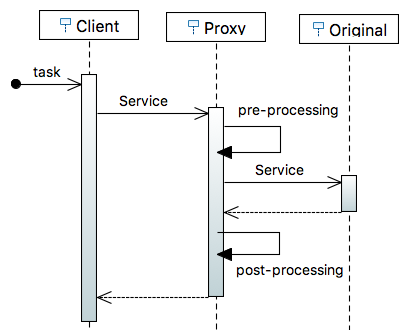
\includegraphics[width=.7\columnwidth]{figure/sequence1.png}
\caption{Process of how proxy pattern handles tasks}
\label{fig:proxyPattern}
\end{figure}


\subsubsection{Reference Patterns}
As mentioned in Section~\ref{sec:background}, the DbC approach considers the two sides of the contract as the caller and the callee (or the client and the server). For this reason, the traditional client-server pattern in the software architecture design is a very good reference pattern. In the client-server pattern, the component types are clients and servers, and the principal connector type for it is a data connector driven by a request/reply protocol used for invoking services~\cite{ii8}. A client is defined as a component that invokes services from a server component. A server is a component that provides services to clients. One component can be both a client and a server. This pattern is widely used as it ``factors out common services which are reusable"~\cite{ii8}. 

We got inspiration also from the Proxy patten for what concerns the 
%Another pattern that I drew lessons from is the Proxy patten. It is not how the components in this pattern distribute, but the way it handles
handling of the invoked service. %that is worthy of learning. 
As shown in Figure~\ref{fig:proxyPattern}, when a client component invokes a service from a server component, the proxy component will make pre-processing for the input and post-processing for the output. The pre-processing and post-processing can serve many purposes including converting formats. The idea is to exploit the pattern for input and output checking and to combine it with the widely approach.  %That is why I think it can also serve as input and output checking. This approach can combine with the Design by Contract approach. 


\subsubsection{Description of the Final Solution}
When combining the DbC approach with the two reference patterns, the most significant point is where to define the pre-conditions, post-conditions, and invariants. Figure~\ref{fig:solution} shows the design for the new components enhanced with DbC and how the components work together. The main processing component is almost the same as the original component. It is responsible for calculating or handling the input data and generating the output data. The newly-built pre-condition, post-condition and invariant components around it are responsible for data check. 

\begin{figure}[t]
\centering
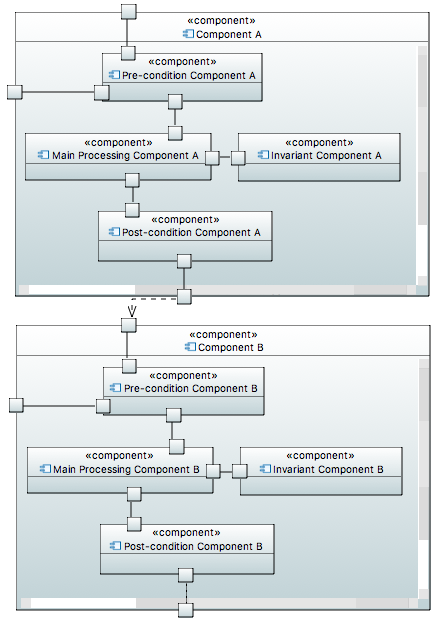
\includegraphics[width=.85\columnwidth]{figure/component11.png}
\caption{Design for AUTOSAR SW-Cs with Design by Contract}
\label{fig:solution}
\end{figure}

In the {\em Pre-condition component}, there is a function that works for checking all the input data. If the input is invalid or erroneous, it can be throw away or, if possible, it can be changed in %make it into 
a default and valid value. How to deal with it depends on the specific requirements. The {\em Pre-condition component} will then give the checked input data to the main processing component for further calculation. In the {\em Invariant component} one or more functions are defined. Each function is used for checking one structure or type in the code of the main processing component. When there is a structure or type in the code, it will invoke the corresponding function to check this structure before using it. In the {\em Post-condition component} there is a function that works for checking all the output data. It will make sure that the output is in the reasonable range. 

Considering how Proxy pattern handles input and output data, the newly-built pre-condition, post-condition and invariant components can be viewed as a proxy component. If one component needs the output data of another component as its input in an AUTOSAR software application, these two components can be seen as a client and a server. Figure~\ref{fig:dataExchange} shows how the input data are handled and exchanged between the components.

\begin{figure}[htb]
\centering
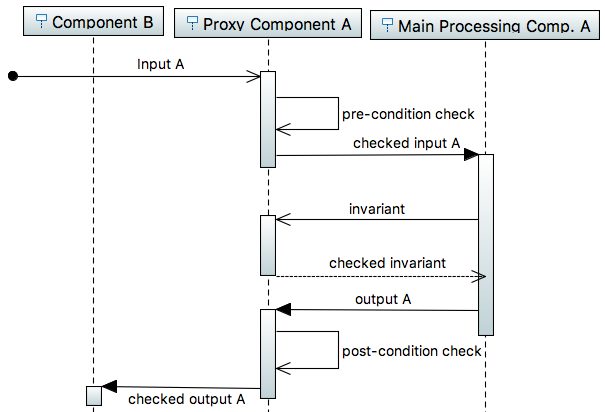
\includegraphics[width=\columnwidth]{figure/sequence2.png}
\caption{How data are handled and exchanged between components}
\label{fig:dataExchange}
\end{figure}

\section{Implementation}\label{sec:implementation}
This section introduces the process of setting up the development environment including exporting the Brake-Pedal-Input-Handler component and Brake-Light-Control component from the Arctic Studio, and importing them into ARUnit. Then, the implementation includes the identification of pre-conditions and post-conditions\footnote{In the considered components there was no need for invariant checks. As the functioning of the invariant component is similar to the functioning of the functions in the pre-condition and post-condition components, this will not affect the evaluation of our solution. In the AUTOSAR software components of other projects or applications, there are structures or types. Therefore invariant component can be used in those software components though it is not used here.}, and the design, modification and testing of the two software components. 

\subsection{Environment Setup and Components Import}
The PC used for the implementation and experimentation uses Windows 7 as the operating system and the two main development tools, Arctic Studio and ARUnit (introduced in Section~\ref{sec:background}), are installed correctly on it. Arctic Studio provides a complete embedded software development environment for automotive embedded software based on AUTOSAR\footnote{\url{http://www.arccore.com/products/arctic-studio}}. %Another development tool, ARUnit, has been introduced in Section~\ref{sec:background}.

Arctic Studio is the original development tool for the existing AUTOSAR SW-Cs. %The whole AUTOSAR software package that was developed in the DEDICATE framework project~\cite{pp} is in this tool. 
%\pat{More information on DEDICATE project} 
It makes the architecture easy to understand and the components easy to recognize and read. Driven by the industrial co-authors, and by reading through the code of the components and the available documentation, we selected the Brake-Pedal-Input-Handler Component and the Brake-Light-Control Component from the applications in this package as the components to be considered for the experiment. These two components are described in Section~\ref{sec:example}.

Arctic Studio and ARUnit are built for different purposes. ARUnit is more efficient for running and testing one single component or certain components. In order to modify and test the two selected components independently from the relevant components in the applications, the ECU, and the real running environment, we exported them from the whole package in Arctic Studio and imported them into ARUnit. The files that we imported into ARUint are the source files of the components and the software component description files of them. ARUnit is then used to generate the run-time environment for them. % according to these files when running them. 
Finally, code files used for testing are built in ARUnit as well. 

%In the software package of the DEDICATE framework project that the company gave me, I did not find a structure or type that should be checked with invariants in the components.\pat{cambia} That is why in the implementation part there are not descriptions about it. 
%As how the functions in the invariant component work is similar to the functions in the pre-condition and post-condition components, it will not affect the verification of this method. In the AUTOSAR software components of other projects or applications, there are structures or types. That means invariant component can be used in those software components though it is not used here.

\subsection{Selected AUTOSAR Software Components}\label{sec:example}
%An AUTOSAR software component is defined as the encapsulation of part of the functionality of the AUTOSAR application~\cite{aa}. An AUTOSAR application is composed of one or several SW-Cs. How to describe the interfaces of these AUTOSAR SW-Cs is defined and standardized within AUTOSAR. Each component can only be distributed to one AUTOSAR ECU. This is the reason why the AUTOSAR SW-C is called as ``Atomic Software Component"~\cite{aa}. AUTOSAR does not prescribe the size of the SW-Cs and how the SW-Cs are implemented. But in order to be able to  integrate several AUTOSAR SW-Cs correctly, one formal and complete description for one SW-C is needed when it is implemented. The description introduces how to configure the infrastructure for the component when building the system. %The introductions to the components that I work on are given below. 
In this section we describe the AUTOSAR software components we selected for the evaluation. These two components have been selected with the support of experts within Volvo AB and they are representative of the set of the existing AUTOSAR software components for the purpose of studying robustness. These components are used in many research projects within Volvo AB. 
%
%\subsubsection{Brake-By-Wire Application}
%In order t
To better understand the functionality of these components % selected AUTOSAR software components, %in this thesis, 
we first introduce the software application that includes them, i.e. the Brake-By-Wire application (BWB). %should be introduced. Here is the Brake-By-Wire application. 

The Brake-By-Wire is an application that is used in several research projects within Volvo AB. %is a research framework %developed by the DEDICATE project~\cite{pp} 
%that 
It implements a brake-by-wire function distributed over five ECUs. It is not the real system that is used in the real trucks. It is proposed to give an example of distributed safety-critical system for validating research projects. The BBW application also includes an environment model of the vehicle in order to simulate the behaviour of the entire vehicle for what concerns acceleration and braking~\cite{pp}. When using this application, the Brake Pedal ECU gets the signal of braking, does the calculation and then sends a corresponding brake force request to each wheel.

\subsubsection{Brake-Pedal-Input-Handler component}
The distribution of the Brake-Pedal-Input-Handler component in the Brake-By-Wire system is shown in Figure~\ref{fig:BPIH}. The function of this component is to convert the hardware pedal input into a pedal position (0-100\%). The input of this component is an integer with 12 bits and the output is a percentage from 0\% to 100\%. It provides input for the Brake-Torque-Calculation component and the Brake-Light-Control component.


\begin{figure}[htb]
\centering
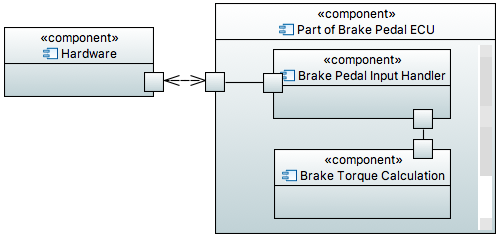
\includegraphics[width=.96\columnwidth]{figure/brakepedal1.png}
\caption{Brake-Pedal-Input-Handler component distribution on ECU.}
\label{fig:BPIH}
\end{figure}

\subsubsection{Brake-Light-Control component}

The distribution of the SW-Cs in the Brake-Lighting application is shown in Figure~\ref{fig:brakelighting}. The Brake-Light-Control component is located on the BrakePedalECU. It inputs vehicle speed and brake pedal position (0-100\%) and outputs ON or OFF for the brake lights according to some rules. The basic rules~\cite{pp} are:

\begin{enumerate}
\item The brake light is always OFF when the pedal input is 0\%.
\item The brake light is always fixed ON whenever the pedal input $>$ 0\% and the vehicle speed is $<$ 10km/h.
\item From 10km/h and above the brake light will blink ON/OFF if emergency braking is active otherwise it is fixed ON.
\end{enumerate}

\begin{figure}[htb]
\centering
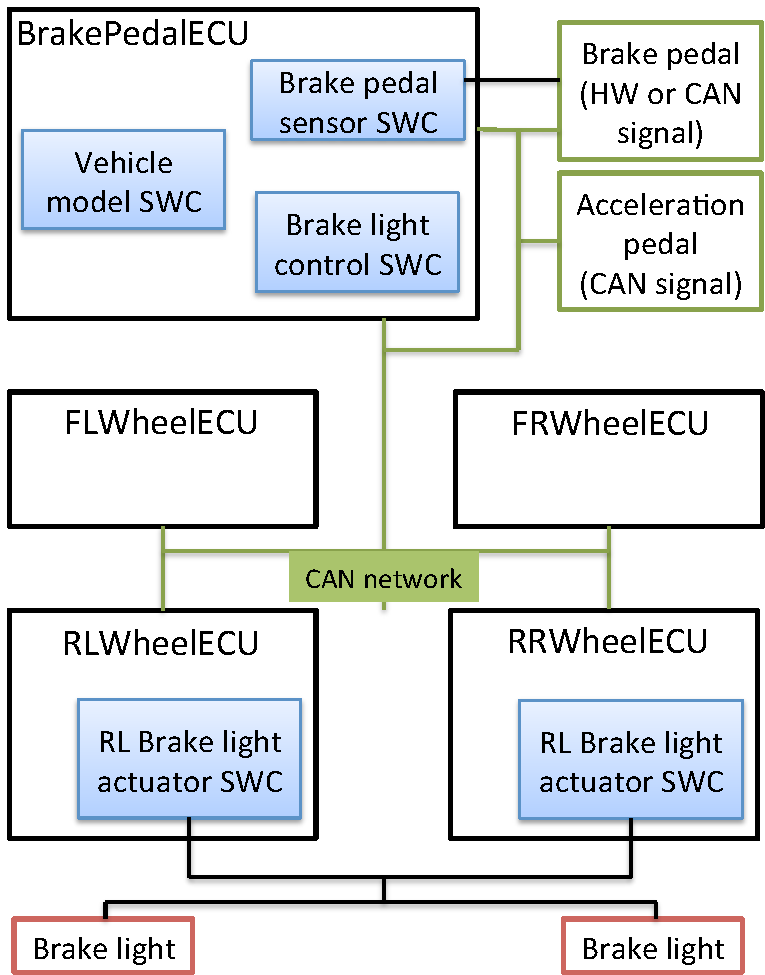
\includegraphics[width=.68\columnwidth]{figure/brakelighting.pdf}
\caption{Brake lighting SW-Cs distribution on ECUs~\cite{pp}}
\label{fig:brakelighting}
\end{figure}

\subsection{Process of Modifying the Brake-Pedal-Input-Handler Component}

In this section, we describe the analysis of the original component, the process of design, the modification and testing of the Brake-Pedal-Input-Handler component according to the Design by Contract approach.

\subsubsection{Issues of the Current Component}
Several issues were raised when reviewing the original component that may threaten the realization of the expected functionality and the robustness of the whole component. One issue is that there are no complete input checks for the component. %Inside t
The component does not handle the input in all the possible ranges of values that are mentioned in the documentation. %DEDICATE framework description \cite{pp}. 
In other words, the input check is too simple to deal with all the possible conditions. 

Another issue is that there is no output check to ensure that the data gotten from the component is completely correct for the next component that uses the data. Although the calculation in this component is not complex, the errors cannot be completely avoided at runtime. That is why output check is necessary.

Finally, other issues concern the internal logic and the readability of the component code. In the original component, the simple and incomplete input checks are mixed with the code that is responsible for the calculation. This makes the code hard to read and understand for developers. This may also threaten the robustness when modifying the code. 

\subsubsection{Identification of Pre-conditions and Post-conditions}

According to the documentation %DEDICATE framework description \cite{pp} 
and the package of all the program code, the Brake-Pedal-Input-Handler component is used to convert the analogue input from the pedal into a pedal position which is from 0\% to 100\%. The pedal provides an analogue input with the range from 10\% to 90\% of supply voltage (5V direct current), which means the voltage is about from 0.5V to 4.5V. If the analogue input is 0-0.5V, it means that it is an open circuit or short to ground. If the analogue input is 4.5-5V, it means that the battery level is too low. %it is short to battery. 
Both of them are errors. For the reason that the AD (Analog-to-Digital) converter of the micro-controller has not been calibrated, this inaccuracy has to be considered when building the software. % \cite{pp}. 
The output from the AD converter is the input for the software component we considered. The input is a 12 bit value, which uses 0 to represent 0V and uses 4095 to represent 5V. Of course, if considering that the input values of the test cases for this component can come also from the ARUnit, the input can possibly be less than 0 or greater than 4095. Thus, input values in these ranges are seen as invalid.

\begin{table}[htb]
\centering
\begin{tabular}{|c|c|c|c|c|c|c|c|}\hline
Range of Input Value\\ \hline
value $<$ 0\\ \hline
0 $<=$ value $<=$ 400\\ \hline
401 $<=$ value $<=$ 499\\ \hline
500 $<=$ value $<=$ 3500\\ \hline
3501 $<=$ value $<=$ 3700\\ \hline
3701 $<=$ value $<=$ 4095\\ \hline
value $>$ 4095\\ \hline
\end{tabular}
\caption{Ranges of input value}
\label{tab:BPIHRanegInput}
\vspace{-.4cm}
\end{table}

Table~\ref{tab:BPIHRanegInput} shows all the possible inputs of the Brake-Pedal-Input-Handler component. What we need to do next is to set contracts for the component. %That is to say, pre-conditions and post-conditions will be discussed in detail. 

When setting pre-condition part of the contracts, the information from requirements specification should be carefully considered to cover all the possible inputs. In this specific example the precondition considers as a valid input only an input value in the range 401 - 3700. 
%Here, pre-condition is that only the input value between 401 and 3700 is seen as valid and faultless. 
When the input value is less than 0 or greater than 4095, it is an invalid input. Input value in this range just appears in the testing environment in ARUnit\footnote{These values should not really come in real environments}. When the input value is in the range of  0-400 and 3701-4095, it is erroneous. Input values in this range represents 0-0.5V or 4.5-5V. They can be generated by the errors of hardware in the vehicles. For the post-condition, it should meet two requirements. Firstly, the output of the software component should be an integer from 0 to 100 to represent values from 0\% to 100\%. Then, the correctness check for the calculation within the component is needed. There are not structures or types used in this component. Hence, we do not need to set invariant checks for them.


\subsubsection{Design and Modification}

The aim of the modified software component is to solve the issues that exist in the original component with the Design by Contract approach. As mentioned in Section~\ref{sec:background}, the separation of the contracts and the component itself is a good practice. The architecture design of the new component is shown in Figure~\ref{fig:BrakePedalComponent}. 

\begin{figure}[htb]
\centering
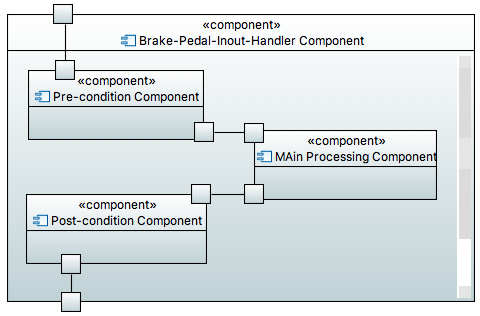
\includegraphics[width=.8\columnwidth]{figure/component222.png}
\caption{Design for the Brake-Pedal-Input-Handler Component.}
\label{fig:BrakePedalComponent}
\end{figure}

In the pre-condition component, there is a function that gets the pedal signal as input and verifies it for the main processing component. Only the valid and faultless data, which are greater than 401 and less than 3700, can enter into the main processing component. The invalid and erroneous data are detected and handled. 
In order to see the testing results intuitively, in our design it directly shows in the console of ARUnit that it is invalid or erroneous. For example, if the input is -100, the console shows it is an invalid input.  But when running in the real ECU, other approaches should be used to handle an invalid or erroneous input because of lack of a screen. The possible approaches may be the correction of the data or getting the next input data after some time. The main processing component works for calculation of the data and giving the results to the post-condition component for checks. The code for data processing in the main processing component is the same of the original component. In the post-condition component, a function used for checking the calculation results of the main processing component is defined. It checks if the calculation is correct and the output is in the range of 0\%-100\%. 

\subsubsection{Test}
In order to get to know if the modified component improves the robustness of the component, a testing program is created for the original component and the modified component in ARUnit. When running the testing program, the input data are sent into the component and the output data are shown on the console in ARUnit through the testing program. For better readability of the output data, some additional comments are attached with the output data to show the status of the calculation. Of course, this is used just in the testing environment to help developing the component and collecting information. In the real ECU, there are not such additional comments at runtime. 

In Table~\ref{tab:BPIHExpectedOutput}, some examples of input data in all possible ranges of the Brake-Pedal-Input-Handler Component are shown. According to the documentation, %DEDICATE framework description~\cite{pp}, 
the expected outputs of the software component are also included to help readers better understanding the testing. 

\begin{table}[htb]
\centering
\begin{tabular}{|c|c|c|}\hline
Range of Input Value & Input Example & Expected Output \\ \hline
value $<$ 0 & -100 & invalid input\\ \hline
0 $<=$ value $<=$ 400 & 200 & erroneous input\\ \hline
401 $<=$ value $<=$ 499 & 450 & 0, successful\\ \hline
500 $<=$ value $<=$ 3500 & 2100 & 53, successful\\ \hline
3501 $<=$ value $<=$ 3700 & 3600 & 100, successful\\ \hline
3701 $<=$ value $<=$ 4095 & 3900 & erroneous input\\ \hline
value $>$ 4095 & 6000 & invalid input\\ \hline
\end{tabular}
\caption{Examples of input for the Brake-Pedal-Input-Handler component and the expected output}
\label{tab:BPIHExpectedOutput}
\vspace{-.4cm}
\end{table}


In the testing period, 70 different input data are tested for both the original component and the modified component. If the output received from the component matches the expected output, we are in the case of a successful running. Referring to the Table~\ref{tab:BPIHExpectedOutput}, the tests that get valid output data such as 0, 53 and 100 are considered as successful tests that can be used by other components. Moreover, also 
%which can be used by other components are seen as successful tests, 
the tests that successfully detect invalid or erroneous inputs are seen as successful tests. The results of the testing are described in Section~\ref{sec:evaluation}. The robustness of the tested software component can be measured in terms of number or percentage of  %seen through how many of the
 test cases that are successful.

\subsection{Process of Modifying the Brake-Light-Control Component}

In this section, we describe the process of modifying the Brake-Light-Control component with the Design by Contract approach. This section emphasizes on the collaboration between the Brake-Light-Control component and the Brake-Pedal-Input-Handler component.

\subsubsection{Analysis and Identification of Pre-conditions and Post-conditions }

The existing issues for the Brake-Light-Control component are similar to the Brake-Pedal-Input-Handler component. It does not have complete input checks for the input data to cover all the possible input data. Some simple input data checks are mixed with the program code. Also, it lacks output checks. The modification for the original component is expected to solve these issues.

The Brake-Pedal-Input-Handler component is used to control the brake lights by the rules described in Section~\ref{sec:example}. Its input should be the pedal position and the vehicle speed. The pedal position is an output of the Brake-Pedal-Input-Handler component. The pedal position should be in the range 0\%-100\%. The range of the vehicle speed depends on different situations. Here, we set the highest vehicle speed as 300 km/h, which is obviously out of the range. Another factor that affects the output of the component is the status of emergency braking. The status of emergency braking can be active or inactive. In order to concentrate on the collaboration of the two modified components, the status of emergency braking is directly sent into the Brake-Light-Control component as another input without being included in the pre-condition. Thus, the pre-condition for this component is that the pedal position should be in the range 0\%-100\% and the vehicle speed should be in the range 0 km/h-300 km/h. For the post-condition, it should check if the calculation in the component is correct.

\subsubsection{Design and Modification}
 The design of the new Brake-Light-Control component is similar to the new Brake-Pedal-Input-Handler component. The pre-condition and post-condition are separated from the main processing component as the pre-condition component and the post-condition component. Figure~\ref{sec:testingEnvironment} shows how these components work together.

\begin{figure}[htb]
\centering
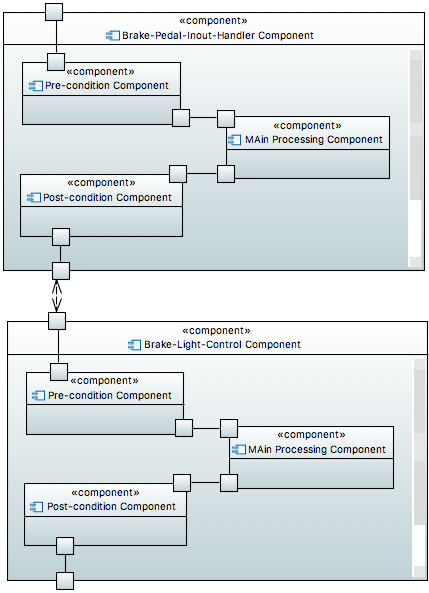
\includegraphics[width=0.9\linewidth]{figure/component33.png}
\caption{Design for the two selected components in the testing environment}
\label{sec:testingEnvironment}
\end{figure}


A function in the pre-condition component of the Brake-Light-Control component gets as input data from the Brake-Pedal-Input-Handler component and other sources, and then verifies the data for the main processing component. Only the input data with pedal position from 0\% to 100\% and vehicle speed from 0 km/h to 300 km/h are valid. The code for data processing in the main processing component is the same of the original component. In the post-condition component, a function used for checking the calculation results of the main processing component is defined. It checks if the status of braking light is correct.



\subsubsection{Test}
In order to know if the two modified components can collaborate with each other and improve the robustness, a testing program is created for the original components and for the modified components in ARUnit. When running the testing program, the input data are sent into both the two components. Data similar to those in Table~\ref{tab:BPIHRanegInput} are passed to the Brake-Pedal-Input-Handler component. Its output data are used as the input data for the Brake-Light-Control component with the vehicle speed and the emergency braking status. The output is the status of the brake lights. It can be ON/OFF/BLINK. Some comments are attached to the output to know which input is detected as invalid or erroneous. 

In Table~\ref{tab:inputData}, some examples of input data are shown. According to the documentation, the expected outputs of the software component are also included to help readers better understanding the testing. 

\begin{table}[htb]\footnotesize
\centering
\begin{tabular}{|p{1.5cm}|c|p{1.9cm}|p{1.9cm}|}\hline
Brake Pedal Input& Vehicle Speed & Emergency Braking Status & Expected Output \\ \hline
2000 & 5 & active & ON\\ \hline
450 & 35 & inactive & OFF\\ \hline
3000 & 35 & active & BLINK\\ \hline
200 & 35 & inactive & erroneous brake pedal input\\ \hline
500 & 400 & inactive & erroneous vehicle speed\\ \hline
\end{tabular}
\caption{Examples of input for the two selected components and the expected output}
\label{tab:inputData}
\vspace{-.4cm}
\end{table}


In the testing period, 30 different sets of input data are tested for both the original components and the modified components. If the output received from the components matches the expected output, it means that it is a successful testing. If it successfully detects the invalid or erroneous input, it is still seen as a successful testing. The results of the performed tests are described in Section~\ref{sec:resultsModified}. The robustness of the tested software component can be measured in terms of number and percentage of successful test cases.

%seen through how many of the test cases are successful.

